\documentclass[12pt]{article}
\pdfoutput=1
\usepackage[T2A]{fontenc}
\usepackage[utf8]{inputenc}
\usepackage[english, russian]{babel}
%\usepackage{NotesTex_rus}
\usepackage{a4wide}
\usepackage{amsmath,amsfonts,amssymb,amsthm,mathtools} 
\usepackage{wasysym}
\usepackage{indentfirst}
\usepackage{a4wide}
\usepackage{mathtools}
\usepackage{dsfont}
\usepackage{float} 
\usepackage{hyperref}


\DeclarePairedDelimiter{\norm}{\lVert}{\rVert} 

\newtheorem{theorem}{Теорема}
\newtheorem{note}{Замечание}
\newtheorem{statement}{Утверждение}
\newtheorem{definition}{Определение}


%Заголовок
%\usepackage{graphix}

\begin{document}
\thispagestyle{empty}
\begin{center}
\vspace{-3cm}

\includegraphics[width=0.5\textwidth]{msu.eps}\\

{\scshape Московский государственный университет имени М.~В.~Ломоносова}\\
Факультет вычислительной математики и кибернетики \\
Кафедра системного анализа

\vfill
{\LARGE Курсовая работа}
\vspace{3cm}

{\Huge\bfseries <<Динамические системы с дискретным временем>>}
\end{center}
\vspace{1cm}
\begin{flushright}
\large
\textit{Студент 315 группы}\\
Г.~А.~Юшков \\
\vspace{5mm}
\textit{Преподаватель}\\
к.ф.-м.н., доцент И.~В.~Востриков
\end{flushright}
\vfill
\begin{center}
Москва, 2022
\end{center}
\makeatother

\newpage
\tableofcontents

\newpage
\section{Постановка задачи}
Даны системы:
$$
    u_{t+1} = u_t^{\frac{5}{2}}e^{-r\sqrt{u_t}}, r > 0, u_t \geqslant 0, \forall t = 0, 1, ...,
$$
$$
    u_{t+1} = u_t^{\frac{5}{2}}e^{-r\sqrt{u_{t-1}}}, r > 0, u_t \geqslant 0, \forall t = 0, 1, ....
$$
Необходимо:
\begin{enumerate}
    \item Найти неподвижные точки.
    \item Исследовать устойчивость неподвижных точек в зависимости от значений параметров.
    \item Проверить существование циклов длиной 2 и 3.
    \item В случае существования цикла длиной 3 построить бифуркационную диаграмму.
    \item Построить график показателя Ляпунова в зависимости от значений параметра.
    \item В случае системы с запаздыванием проверить возможность возникновения бифуркации Неймарка-Сакера. 
\end{enumerate}

\newpage
\section{Исследование первой системы}
\subsection{Неподвижные точки системы}
Рассмотрим дискретную динамическую систему:
\begin{equation}
    u_{t+1} = f(u_t), ~ u_t \in \mathbb{R}, f: \mathbb{R} \rightarrow \mathbb{R}, \label{eq:defsystem1}
\end{equation}
или, в других обозначениях:
\begin{equation}
    u \mapsto f(u), ~ u \in \mathbb{R}, f: \mathbb{R} \rightarrow \mathbb{R}. \label{eq:defsystem2}
\end{equation}
\begin{definition}
    Множество всевозможных состояний $u_t$ называется \textit{пространством состояний}(или \textit{фазовым пространством} системы (\ref{eq:defsystem1}).
\end{definition}
\begin{definition}
    Множество точек $u_t, t = 0, 1, ...$ называется \textit{траекторией} (или \textit{орбитой}) системы (\ref{eq:defsystem1}).
\end{definition}
\begin{definition}
    Неподвижными точками системы (\ref{eq:defsystem1}) называются такие точки пространства состояний $u^*$, что $f(u^*) = u^*$.  
\end{definition}
Будем исследовать следующую систему:
$$
    u_{t+1} = u_t^{\frac{5}{2}}e^{-r\sqrt{u_t}}, ~ r > 0, u_t \geqslant 0, \forall t = 0, 1, ...,
$$
\subsection{Нахождение неподвижных точек}
Для нахождения неподвижных точек будем искать точки пересечения графиков $f(u) = u^{\frac{5}{2}}e^{-r\sqrt{u}}$ и $g(u) = u$.
Очевидно, что при любом значении параметра $r$ точка $u = 0$ является неподвижной. Дальнейшее исследование показывает, что неподвижных точек может быть от 1 до 3 (с учётом нуля). Случай двух неподвижных точек возможен при касании $f(u)$ и $g(u)$. При увеличении значении параметра $r$, выше того, при котором происходит касание, график $f(u)$ быстрее "прижимается" к оси абсцисс и единственной неподвижной точкой остаётся нуль. При уменьшении же, наоборот, появляется часть графика $f(u)$, лежащая над графиком $g(u)$. Из соображений непрерывности это приводит к появлению двух дополнительных (отличных от нуля) неподвижных точек. Определим условие касания:
\begin{theorem}
    Если кривые заданы явным уравнением $y = f(x)$, $y = g(x)$, то они касаются в точке с абсциссой $x_0$ тогда и только тогда. когда:
    \begin{equation}
        \begin{cases}
            f(x_0) = g(g_0),\\
            f'(x_0) = g'(x_0).
        \end{cases}
    \end{equation}
\end{theorem}
Воспользуемся теоремой для посика точки касания и требуемого значения $r$.
\begin{equation}
    \begin{cases}
        f(u) = g(u),\\
        f'(u) = g'(u)
    \end{cases}
\end{equation}
Решая систему элементарными методами, получаем:
\begin{equation}
    \begin{cases}
        r = \frac{3}{e},\\
        u = e^2.
    \end{cases}
\end{equation}
Получаем следующую структуру расположения неподвижных точек в зависимости от параметра $r$:
\begin{enumerate}
    \item При $r \in \left(0, \frac{3}{e}\right)$: есть 3 неподвижные точки: $u_1 = 0$, $u_2 \in (0, e^2)$, $u_3 > e^2$.
    \item При $r = \frac{3}{e}$: есть 2 неподвижные точки: $u_1 = 0$ и $u_2 = e^2$.
    \item При $r > \frac{3}{e}$: есть единственная неподвижная точка: $u_1 = 0$.
\end{enumerate}
\begin{figure} [H]
    \begin{center}
    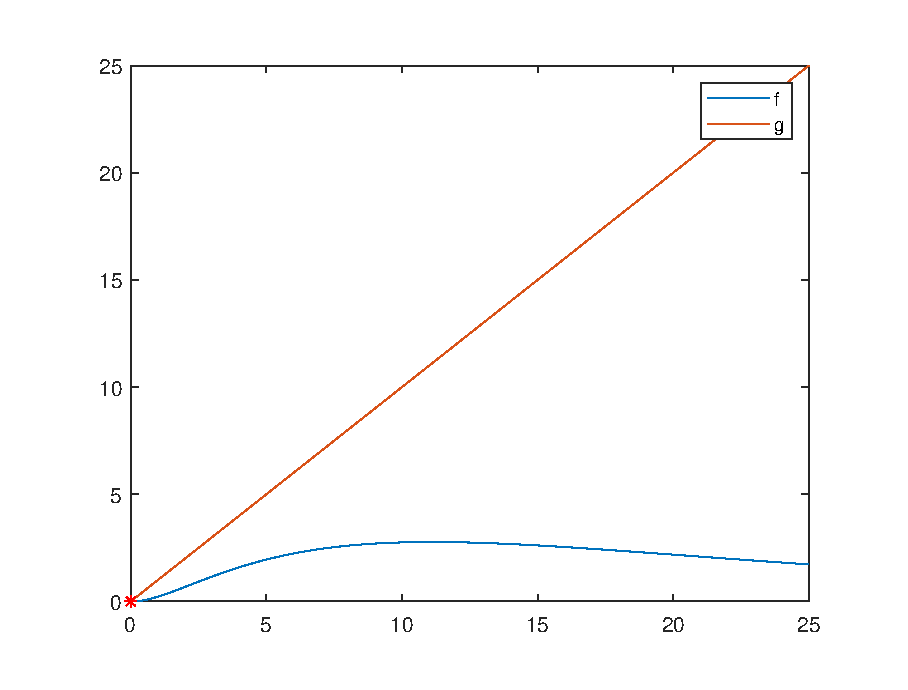
\includegraphics[width=0.7\textwidth]{root1.eps}
    \caption{1 корень. r = 1.5}
    \label{pic1}
    \end{center}
\end{figure}
\begin{figure} [H]
    \begin{center}
    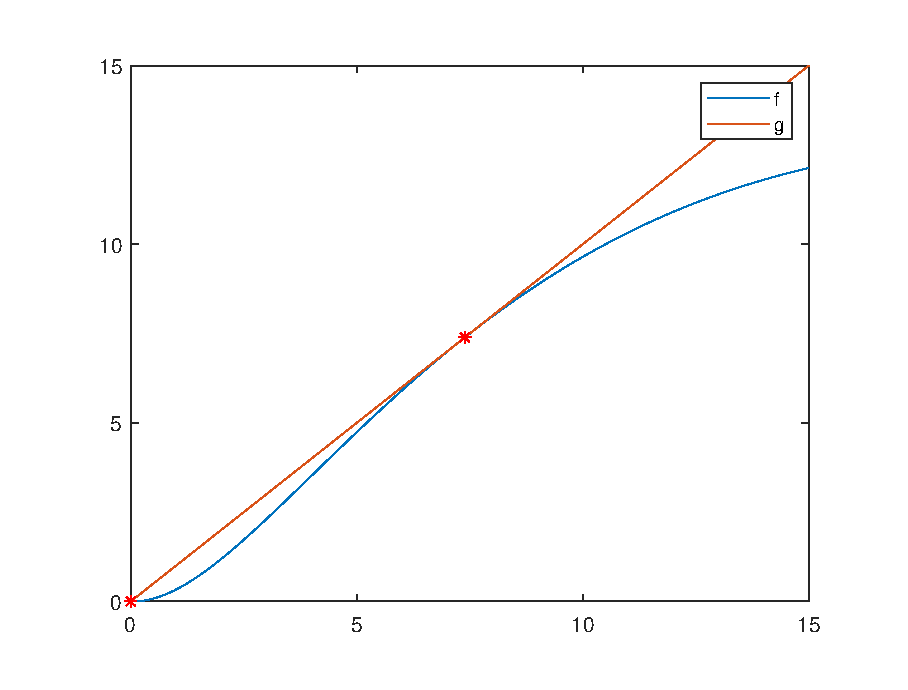
\includegraphics[width=0.7\textwidth]{root2.eps}
    \caption{2 корня. r = $\frac{3}{e}$}
    \label{pic2}
    \end{center}
\end{figure}
\begin{figure} [H]
    \begin{center}
    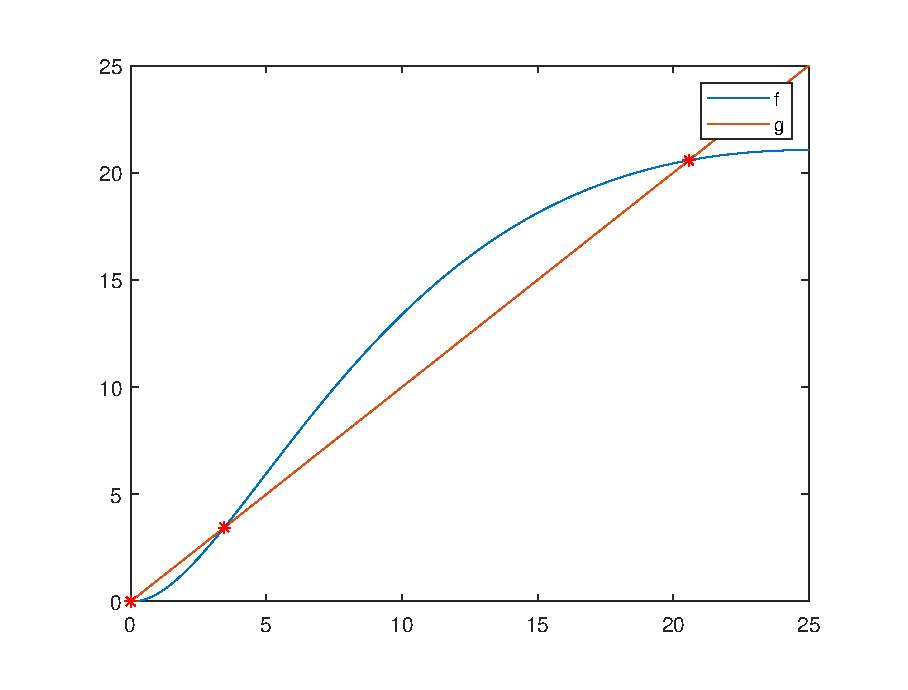
\includegraphics[width=0.7\textwidth]{root3.eps}
    \caption{3 корня. r = 1}
    \label{pic3}
    \end{center}
\end{figure}
\subsection{Устойчивость неподвижных точек}
\begin{definition}
    Неподвижная точка $u^*$ отображения (\ref{eq:defsystem2}) называется \textit{устойчивой по Ляпунову}, если $\forall \epsilon > 0$ существует такое $\delta > 0$, что для любых начальных данных $u_0$ из $\delta-$окрестности точки $u^*$ вся траектория системы $u_t$, $t = 0, 1, ...$ содержится в $\epsilon-$окрестности точки $u^*$. Если, кроме того, \[\lim_{t \rightarrow \infty} f(u_t) = u^*,\] то точка $u^*$ называется \textit{асимптотически устойчивой}.  
\end{definition}
Справедливо следующее утверждение:
\begin{statement}
    Пусть $u^*$ — неподвижная точка отображения (\ref{eq:defsystem2}) и $f$ обратима в малой окрестности $u^*$. Тогда $u^*$ асимптотически устойчива, если $|f_u(u^*)| < 1$, и неустойчива, если $|f_u(u^*)| > 1$. \label{st1}
\end{statement}
Разберём случаи по значению параметра $r$.
\begin{enumerate}
    \item $r > \frac{3}{e}$. Тогда существует единственная неподвижная точка $u_1 = 0$. $f'(0) = 0$, значит, точка 0 - асимптотически устойчива.
    \item $r = \frac{3}{e}.$ Тогда существуют 2 неподвижные точки: $u_1 = 0$, $u_2 = e^2$. $f'(u_1) = 0, f'(u_2) = 1$ (второе равенство вытекает из касания в $u_2$ функций $f$ и $g$). В данном случае ничего нельзя сказать об устойчивости второй неподвижной точки, используя лишь методы линейного анализа.
    \item $r < \frac{3}{e}$. Тогда существуют 3 неподвижные точки: $u_1 = 0$, $u_2 < e^2$, $u_3 > e^2$. Про $u_1$ уже всё известно, разберёмся с $u_2, u_3$.
    \begin{equation}
        f'(u) = \frac{u^\frac{3}{2}e^{-r\sqrt{u}}}{2}(5 - r\sqrt{u}).
    \end{equation}
    В неподвижных точках выполнено равенство: $f(u) = g(u)$, которое удобно применять в виде:
    \begin{equation}
        u^\frac{3}{2}e^{-r\sqrt{u}} = 1.
    \end{equation}
    Для точки $u_2$ выполнено неравенство: $u_2 < e^2$ $\Rightarrow$ $\sqrt{u_2} < e$. Учитывая то, что $r < \frac{3}{e}$, получаем:
    \begin{equation}
        f'(u_2) > \frac{1}{2}(5 - \frac{3}{e}e) = 1.
    \end{equation}
    Значит, точка $u_2$ неустойчива. ерейдём к исследованию $u_3$.
    \begin{equation}
        f'(u_3) = \frac{u_3^\frac{3}{2}e^{-r\sqrt{u_3}}}{2}(5 - r\sqrt{u_3}).
    \end{equation}
    \begin{center}
        $\Updownarrow$
    \end{center}
    \begin{equation}
        f'(u_3) = \frac{5 - r\sqrt{u_3}}{2}.
    \end{equation}
    Достаточным условием асимптотической устойчивости является: $|f'(u_3)| < 1$, откуда вытекает:
    \begin{equation}
        \begin{cases}
            5 - r\sqrt{u_3} < 1,\\
            5 - r\sqrt{u_3} > -1.
        \end{cases}
    \end{equation}
    Получаем условие на асимптотическую устойчивость точки $u_3$: $r\sqrt{u_3} \in (4, 6)$.
    \begin{center}
        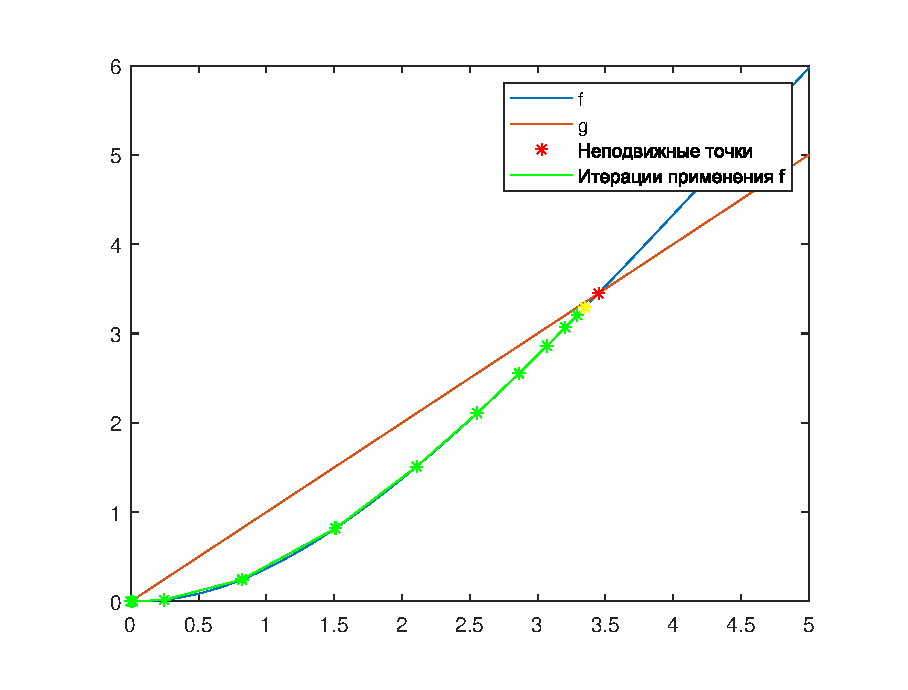
\includegraphics[width=0.7\textwidth]{stability.eps}
        \caption{Устойчивость/неустойчивость в случае a = 1}
        \label{pic4}
    \end{center}
\end{enumerate}

\newpage
\subsection{Существование циклов длины 2, 3}
\begin{definition}
\textit{Циклом длины k} системы (\ref{eq:defsystem1}) называется множество различных точек $u_1, u_2, ..., u_k$ таких, что
$$
    u_2 = f(u_1), ..., u_k = f(u_{k-1}), u_1 = f(u_k).
$$
\end{definition}
Упорядочим все натуральные числа следующим образом:
$$
    3 \succ 5 \succ 7 \succ ... \succ
$$
$$
    \succ 2\cdot 3 \succ 2 \cdot 5 \succ 2 \cdot 7 \succ ... \succ
$$
$$
    \succ 2^2\cdot 3 \succ 2^2 \cdot 5 \succ 2^2 \cdot 7 \succ ... \succ
$$
$$
    \succ ... \succ
$$
$$
    \succ 2^3 \succ 2^2 \succ 2 \succ 1.
$$
\begin{theorem}
    (Шарковский). Пусть $f:\mathbb{R} \rightarrow \mathbb{R}$ — непрерывное отображение, и пусть $f$ имеет цикл длины $k$. Тогда $f$ имеет цикл длины $m$ для всех таких $m$, что $k \succ m$ в указанном выше порядке. \label{th1}
\end{theorem}
Покажем, что существует цикл длины 3. Для этого найдём решение системы:
\begin{equation}
    \begin{cases}
        f^3(u,r) = u, \\
        \frac{df^3(u,r)}{du} = 1, 
    \end{cases}
    \text{где } f^3 = f \circ f \circ f.
\end{equation}

Решим систему численно в среде MATLAB. $r = 0.45, u_0 = 16.3107$.
\begin{figure} [H]
    \begin{center}
    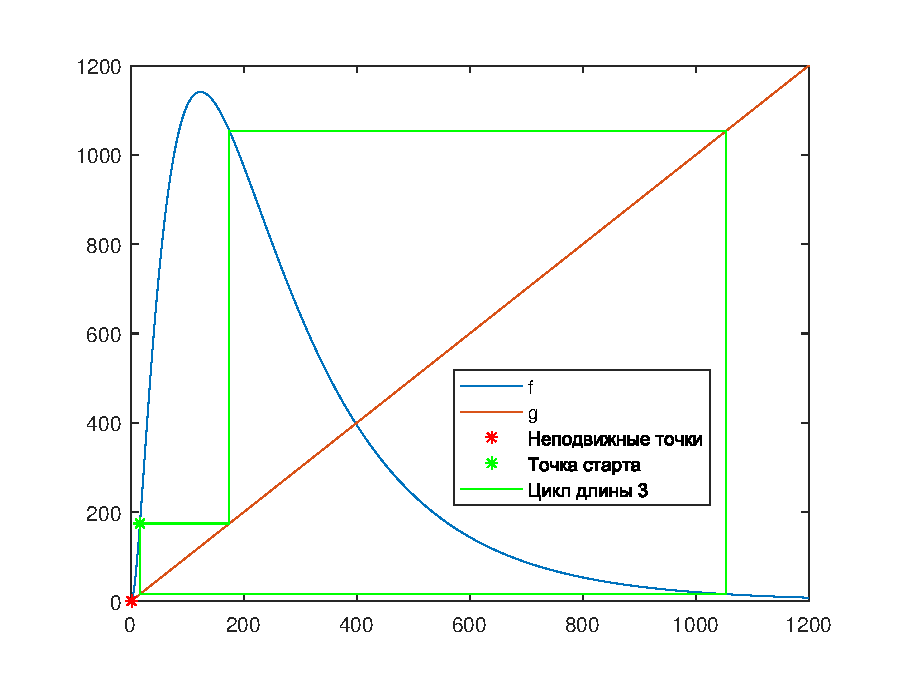
\includegraphics[width=0.7\textwidth]{cycle3.eps}
    \caption{Цикл длины 3. r = 0.45, $u_0 = 16.3107$}
    \label{pic5}
    \end{center}
\end{figure}
Значит, по теореме Шарковского, у системы есть циклы любой длины. Например, для цикла длины 2: $r = 0.45, u_0 = 54.8703$.
\begin{figure} [H]
    \begin{center}
    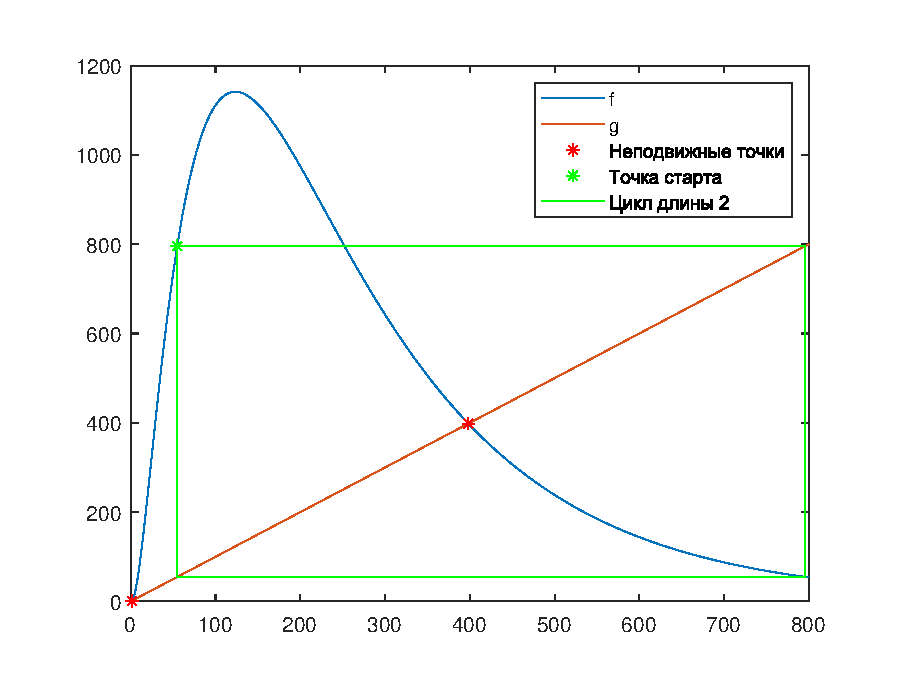
\includegraphics[width=0.7\textwidth]{cycle2.eps}
    \caption{Цикл длины 2. r = 0.45, $u_0 = 54.8703$}
    \label{pic6}
    \end{center}
\end{figure}
\subsection{Бифуркационная диаграмма}
\begin{definition}
    Две дискретные динамические системы \textit{топологически эквивалентны}, если они имеют равное количество неподвижных точек одинакового характера, расположенных в одинаковом порядке на фазовой прямой. При этом фазовые портреты топологически эквивалентных систем также называются \textit{топологически эквивалентными}.
\end{definition}
\begin{definition}
    Появление топологически неэквивалентных фазовых портретов при изменении параметров динамической системы называется \textit{бифуркацией}.
\end{definition}
\begin{definition}
    \textit{Бифуркационной диаграммой} динамической системы называется разбиение пространства параметров на максимальные связные подмножества, которые определяются соотношениями топологической эквивалентности и рассматриваются вместе с фазовыми портретами для каждого элемента разбиения.
\end{definition}
Покажем бифуркационную диаграмму для начального приближения $u_0 = 100$, количества итераций для "сходимости" $n_1 = 600$, количества последующих итераций (отмеченных на графике в виде точек $(r, u_t)$ $n_2 = 200$. Стартовое значение $r$ возьмём $r = 0.1$, конечное - $r = 1$, шаг: $\delta = 0.005$.
\begin{figure} [H]
    \begin{center}
    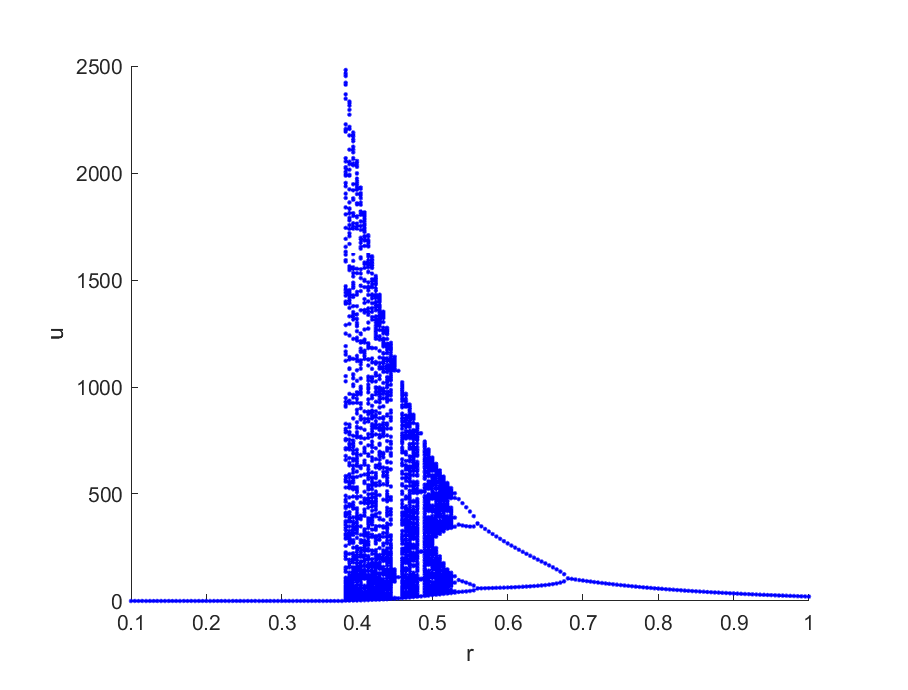
\includegraphics[width=0.7\textwidth]{bifurc.eps}
    \caption{Бифуркационная диаграмма. $u_0 = 100, r_{min} = 0.1, r_{max} = 1, \delta = 0.005, n_1 = 600, n_2 = 200$}
    \label{pic7}
    \end{center}
\end{figure}
\subsection{Показатель Ляпунова}
\begin{definition}
    Пусть $f: \mathbb{R} \rightarrow \mathbb{R}$ — гладкое отображение. Показателем Ляпунова траектории $u_1, u_2, ...$ называется величина:
$$
    h(u_1) = \lim_{n \rightarrow \inf} \frac{\ln{|f'(u_1)|} + \ln{|f'(u_2)|} + ... + \ln{|f'(u_n)|}}{n},
$$
если этот предел существует.
\end{definition}
\begin{definition}
    Орбиту $\{u_i\}^{\inf}_{i=1}$ дискретной системы $u_{t+1} = f(u_t)$ назовём хаотической, если эта орбита ограничена, не стремится к периодической траектории и её показатель Ляпунова $h(u_1)$ больше нуля. \label{def:chaotic} 
\end{definition}
Построим график зависимости показателя Ляпунова от параметра $r$. Возьмём параметры: $u_0 = 35$, $r$ изменяется от значения $0.1$ до $1$ с шагом $\delta = 0.005$, $n = 1000$ (Рис. \ref{pic8}).
\begin{figure}[H]
    \begin{center}
    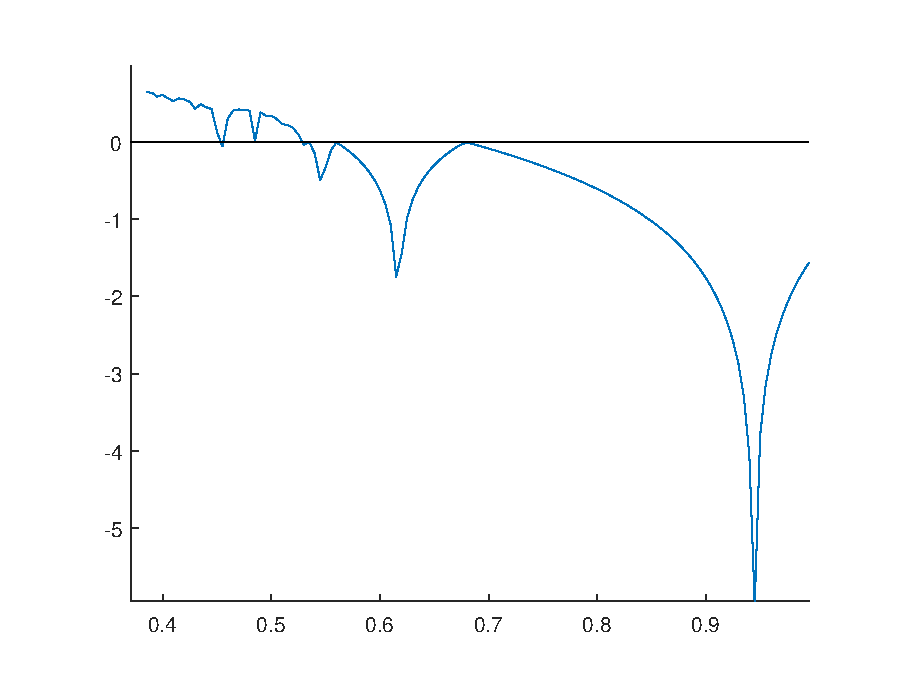
\includegraphics[width=0.7\textwidth]{lyapunov.eps}
    \caption{Зависимость показателя Ляпунова от параметра $r$.}
    \label{pic8}
    \end{center}
\end{figure}
Видно, что при малых значениях $r$ на графике нет значений. Это объясняется тем, что в какой-то момент $u_t = 0$, а ноль - асимптотически устойчивая точка. Таким образом, выражение под знаком предела в определении функции Ляпунова становится равно $\infty$. Это объясняет отсутствие части графика.\\
Показатель Ляпунова является легко вычислимым признаком хаотического поведения. Если $h(u) > 0$, то близкие траектории разбегаются, и в системе может наблюдаться хаотическое поведение. Из графика видно, что на некоторых интервалах в системе наблюдается хаотическое поведение. Интервалы с $h(u) < 0$ соответствуют циклам с небольшим периодом.

\newpage
\section{Исследование второй системы}
\subsection{Неподвижные точки системы}
Рассмотрим систему с запаздыванием:
$$
    u_{t+1} = u_t^{\frac{5}{2}}e^{-r\sqrt{u_{t-1}}}, r > 0, u_t \geqslant 0, \forall t = 0, 1, ....
$$
Перепишем её в другом виде, чтобы избавиться от запаздывания:
\begin{equation}
    \begin{cases}
        u_{t+1} = f(u_t, v_t) = u_t^{\frac{5}{2}}e^{-r\sqrt{v_t}}, \\
        v_{t+1} = g(u_t, v_t) = u_t. \label{cs1}
    \end{cases}
\end{equation}
\begin{definition}
    Точка $u^* \in \mathbb{R}$ является \textit{неподвижной точкой} системы
    $$
        u_{t+1} = f(u_t, u_{t-1}), u_t \in \mathbb{R}, f: \mathbb{R}^2 \rightarrow \mathbb{R},
    $$
    если $f(u^*, u^*) = u^*$.
\end{definition}
Задача сводится нахождению решений следующей системы:
\begin{equation}
    \begin{cases}
        u^* = (u^*)^{\frac{5}{2}}e^{-r\sqrt{u^*}}, \\
        u^* = u^*.
    \end{cases}
\end{equation}
Второе уравнение обращается в тождество, а первое уравнение было рассмотрено при исследовании первой системы. Получим три случая:
\begin{enumerate}
    \item $r > \frac{3}{e}$. Тогда существует единственная неподвижная точка $u_1 = 0$.
    \item $r = \frac{3}{e}$. Тогда есть 2 неподвижные точки: $u_1 = 0$ и $u_2 = e^2$.
    \item $r \in \left(0, \frac{3}{e}\right)$.Тогда есть 3 неподвижные точки: $u_1 = 0$, $u_2 \in (0, e^2)$, $u_3 > e^2$.
\end{enumerate}

\newpage
\subsection{Устойчивость неподвижных точек}
\begin{theorem}
    Пусть дана динамическая система с дискретным временем:
    $$
        u_{t+1} = f(u_t), u_t \in \mathbb{R}^n, f \text{ — гладкое отображение } \mathbb{R}^n \rightarrow \mathbb{R}^n.
    $$
    Тогда неподвижная точка $u^*$ асимптотически устойчива, если все собственные значения $\lambda_1, \lambda_2, ..., \lambda_n$ матрицы Якоби функции $f(u)$, вычисленные в точке $u^*$, таковы, что $|\lambda_i| < 1$, $i = 1, ..., n$. Если хотя бы одно собственное значение $\lambda_i$ таково, что $|\lambda_i| > 1$, то неподвижная точка $u^*$ неустойчива. \label{th2}
\end{theorem}
Рассмотрим матрицу Якоби для системы (\ref{cs1}):
$$
J(u,v) = 
\begin{bmatrix}
    \frac{5}{2}u_t^{\frac{3}{2}}e^{-r\sqrt{v_t}} & \frac{-r}{2\sqrt{v_t}}u_t^{\frac{5}{2}}e^{-r\sqrt{v_t}}\\
    1 & 0
\end{bmatrix}.
$$

\begin{enumerate}
    \item $r > \frac{3}{e}$. Исследуем $u_1 = 0$. 
$$
J(0, 0) = 
\begin{bmatrix}
    0 & 0\\
    1 & 0
\end{bmatrix}.
$$
    Собственные значения: $\lambda_{1,2} = 0$. Точка 0 - асимптотически устойчива.
    \item $r = \frac{3}{e}$. Исследуем $u_2 = e^2.$
$$
J(e^2, e^2) = 
\begin{bmatrix}
    \frac{5}{2} & \frac{-3}{2}\\
    1 & 0
\end{bmatrix}.
$$
    Характеристическое уравнение: $(\frac{5}{2} - \lambda)(-\lambda) + \frac{3}{2} = 0$.\\
    Собственные значения:
    \begin{cases}
        \lambda_1 = 1.5,\\
        \lambda_2 = 1.
    \end{cases}
    Значит, неподвижная точка $(e^2, e^2)$ яыляется неустойчивой.
    \item $r < \frac{3}{e}$. Исследуем $u_2 < e^2.$
    Воспользуемся её неподвижностью: она является корнем уравнений: $f(u) = u$ и $f'(u) = 1$ (из первой системы). Тогда её матрица Якоби примет вид:
$$
    J(u_2,u_2) = 
\begin{bmatrix}
    \frac{5}{2} & \frac{-r\sqrt{u_2}}{2}\\
    1 & 0
\end{bmatrix}.
$$
    Характеристическое уравнение: $(\frac{5}{2} - \lambda)(-\lambda) + \frac{r\sqrt{u_2}}{2} = 0$.\\
    Собственные значения: $\lambda_{1,2} = \frac{5 \pm \sqrt{25 - 4r^2u_2}}{4}$. \\
    Из условий случая получаем: $r^2u_2 < \frac{9}{e^2}e^2 = 9$. Отсюда вытекает, что подкоренное выражение неотрицательно. Тогда собственное значение, в котором корень берётся со знаком "плюс" будет заведомо больше единицы. Значит, точка $u_2$ является неустойчивой.\\
    Применяя аналогичные рассуждения, можно показать, что точка $u_3$ также является неустойчивой.
\end{enumerate}

\begin{figure}[H]
    \begin{center}
    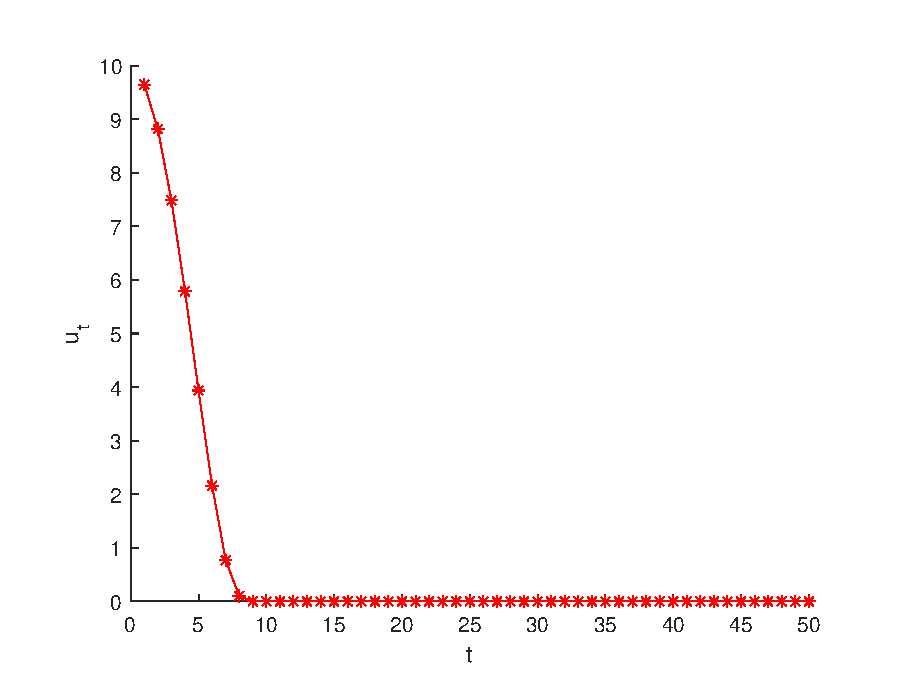
\includegraphics[width=0.7\textwidth]{stability2.eps}
    \caption{Устойчивость нуля во второй системе. $u_0 = u_1 = 10, r = \frac{3}{e}$.}
    \label{pic9}
    \end{center}
\end{figure}

\begin{figure}[H]
    \begin{center}
    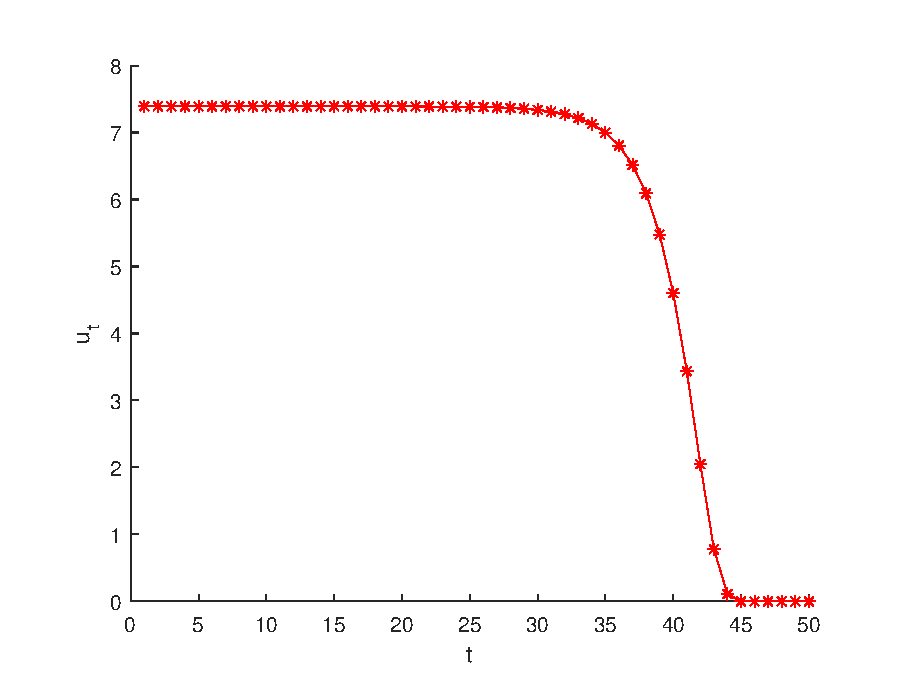
\includegraphics[width=0.7\textwidth]{stability3.eps}
    \caption{Неустойчивость $e^2$ во второй системе. $u_0 = u_1 = 7.39, r = \frac{3}{e}$.}
    \label{pic10}
    \end{center}
\end{figure}

\newpage
\subsection{Бифуркация Неймарка-Сакера}
\begin{definition}
    Бифуркацией положения равновесия в системе (\ref{cs1}), соответствующая появлению собственных значений $|\lambda_1| = |\lambda_2| = 1, \lambda_1 = \bar{\lambda_2}$, называется бифуркацией Неймарка-Сакера.
\end{definition}
Как было показано в пункте про устойчивость неподвижных точек, условия на собственные значения $\lambda_{1,2}$ из определения бифуркации Неймарка-Сакера не выполняются ни для одной из неподвижных точек при всех возможных значениях $r > 0$. Значит, бифуркацию Неймарка-Сакера в данном случае не может возникнуть.

\newpage
\begin{thebibliography}{9}
    \bibitem[1]{} А.\,C.~Братусь, А.\,С.~Новожилов, А.\,П.~Платонов. Динамические системы и модели биологии. — М.: ФИЗМАТЛИТ, 2010.
\end{thebibliography}
\end{document}